\documentclass[11pt,letterpaper]{article}
\usepackage[utf8]{inputenc}

%----- Configuración del estilo del documento------%
\usepackage{epsfig,graphicx}
\usepackage[left=2cm,right=2cm,top=1.8cm,bottom=2.3cm]{geometry}
\usepackage{fancyhdr}
\usepackage{lastpage}

\usepackage{xcolor}
\usepackage{soul}
\newcommand{\mathcolorbox}[2]{\colorbox{#1}{$\displaystyle #2$}}

%Color bibi
\definecolor{bibi}{RGB}{0,103,148}
% Otros colores

\usepackage{cite}
\usepackage{multicol}
\setlength{\columnsep}{1.5cm}
\setlength{\columnseprule}{.5pt}

\pagestyle{fancy}
\fancyhf{}
\rfoot{\textit{Página \thepage \hspace{1pt} de \pageref{LastPage}}}

%------ Paquetes matemáticos básicos --------%
\usepackage{amsmath}
\usepackage{amssymb}
\usepackage{amsthm}

\begin{document}
%------ Encabezado -------- %
\begin{center}
    \begin{minipage}{3cm}
    	\begin{center}
    		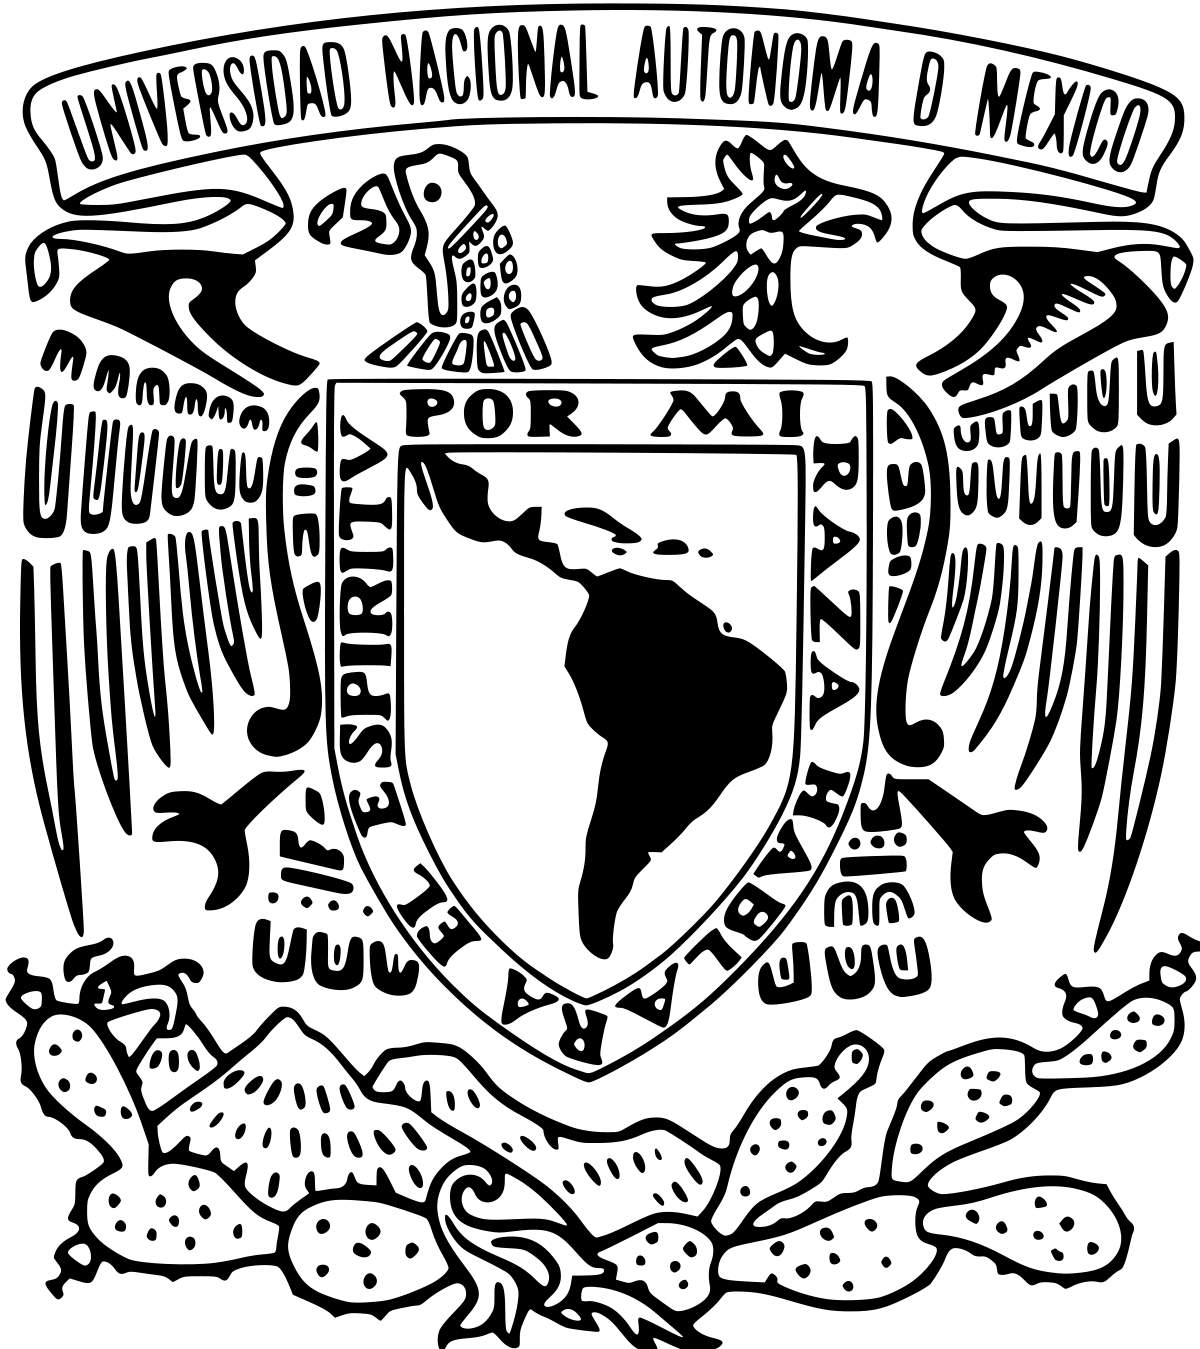
\includegraphics[height=3.4cm]{src/Img/Logo_UNAM.png}
    	\end{center}
    \end{minipage}\hfill
    \begin{minipage}{10cm}
    	\begin{center}
    	\textbf{\large Universidad Nacional Autónoma de México}\\[0.1cm]
        \textbf{Facultad de Ciencias}\\[0.1cm]
        \textbf{Análisis de Algoritmos  $|$ 7083}\\[0.1cm]
        Tarea 3 : $|$ Programacion Dinamica\\[0.1cm]
        Sosa Romo Juan Mario $|$ 320051926 \\[0.1cm]
        25/09/24
    	\end{center}
    \end{minipage}\hfill
    \begin{minipage}{3cm}
    	\begin{center}
    		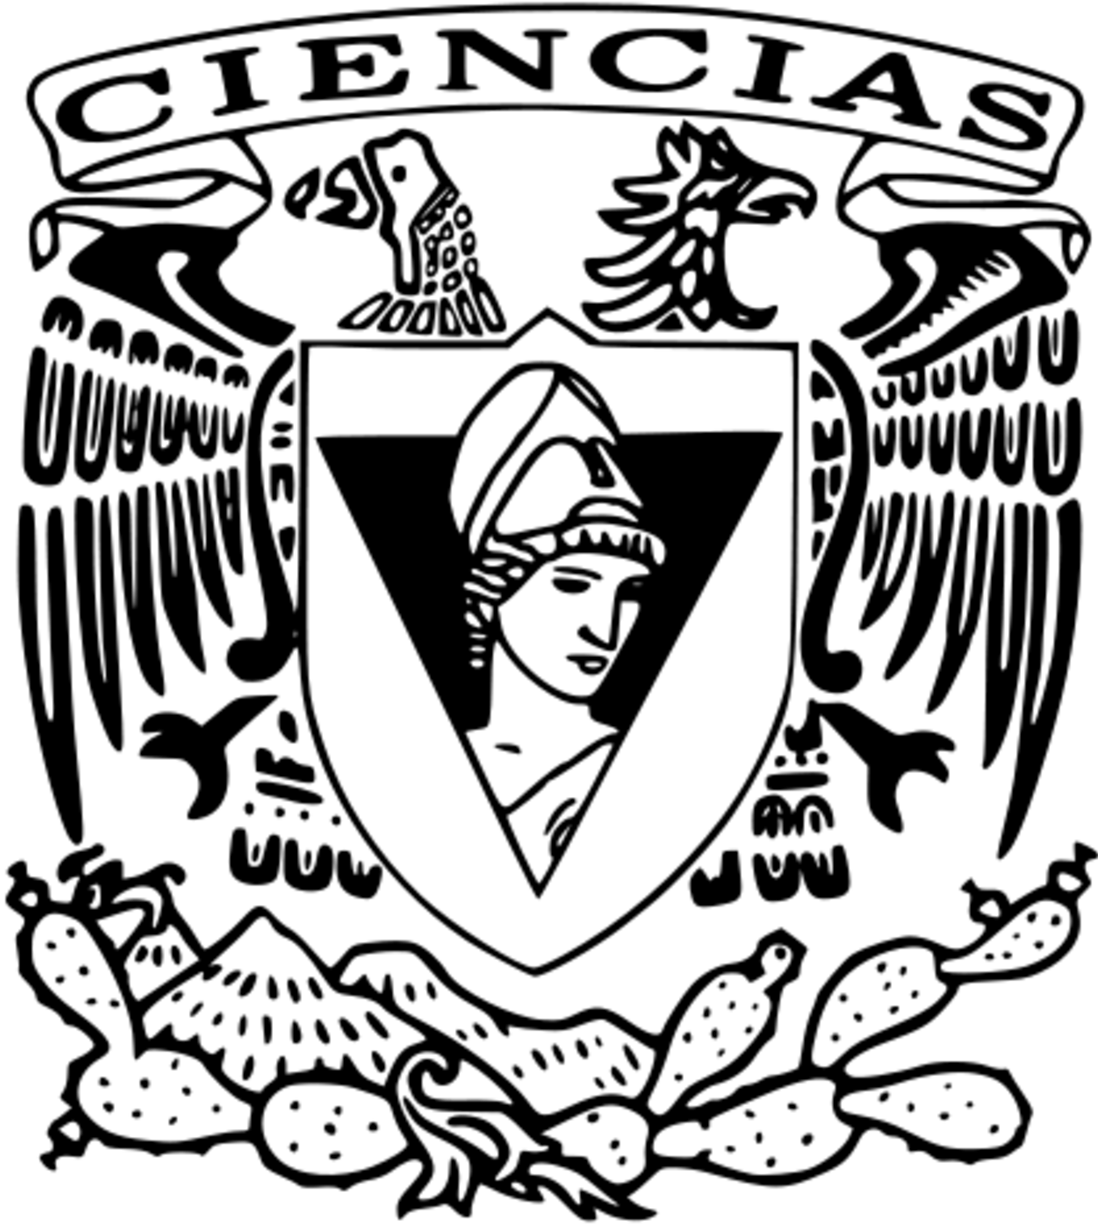
\includegraphics[height=3.4cm]{src/Img/Logo_FC.png}
    	\end{center}
    \end{minipage}
\end{center}


\rule{17cm}{0.1mm}


%------ Ejercicios -------- %
\begin{enumerate}
    \item \textbf{
    Un algoritmo glotón para regresar el cambio
    de n unidades usando el mínimo número de 
    monedas es el siguiente: Dar al cliente una
    moneda de mayor denominación, digamos d.
    Repite lo anterior para regresar el cambio 
    de n-d unidades.
}
\vspace{.3cm}

\textbf{
    Para cada una de las siguientes denominaciónes,
    determina si el algoritmo greedy antes mecionado
    mínimiza el número de monedas para dar el cambio.
    Si es así pruébalo, y si no lo es muestra un 
    contraejemplo.
}\vspace{.2cm}

\textcolor{red}{Esta probablemente no salio, si quiere no la califique pero la intente por si viene en el examen :v}
    \item \textbf{
    Construya el árbol de Huffman para codificar el siguiente texto:
    \begin{center}
        "El azote, hijo mío, se inventó para castigar afrontando al racional y para avivar la pereza del bruto que carece de razón; pero no para el niño decente y de vergüenza que sabe lo que le importa hacer y lo que nunca debe ejecutar, no amedrentado por el rigor del castigo, sino obligado por la persuasión de la doctrina y el convencimiento de su propio interés."
    \end{center}
}\vspace{.2cm}

No voy a explicar el algoritmo de Huffman, pues se vio en clase pero voy a hacer el procedimiento y luego mostrar con un árbol de Huffman online que esta bien hecho. \vspace{.2cm}

\textcolor{bibi}{Creamos el arbol de Huffman}
\begin{quote}
    \begin{itemize}
        \item \textbf{Paso 1:} Contamos la frecuencia de cada letra en el texto. (puede cambiar un poquito si consideras tabuladores o si yo conte mal xd)

        \begin{align*}
            \char`_ &: 65 \\
            e &: 39 \\
            a &: 34 \\
            o &: 27 \\
            r &: 25 \\
            n &: 21 \\
            i &: 17 \\
            l &: 15 \\
            t &: 13 \\
            d &: 13 \\
            c &: 12 \\
            p &: 11 \\
            s &: 9 \\
            u &: 9 \\
            v &: 5 \\
            g &: 5 \\
            z &: 4 \\
            , &: 4 \\
            m &: 4 \\
            y &: 4 \\
            b &: 4 \\
            q &: 4 \\
            \text{ó} &: 3 \\
            h &: 2 \\
            j &: 2 \\
            E &: 1 \\
            \text{í} &: 1 \\
            f &: 1 \\
            ; &: 1 \\
            \text{ñ} &: 1 \\
            \text{ü} &: 1 \\
            \text{é} &: 1 \\
            . &: 1 \\
        \end{align*}
        \item \textbf{Paso 2:} Creamos una lista con los nodos de cada letra y su frecuencia. (este paso literalmente solo es hacer eso entonces no muestro nada)
        \item \textbf{Paso 3:} Tomamos 2 arboles con las frecuencias mas bajas y los unimos en un nuevo arbol con la suma de las frecuencias, la raiz de este nuevo arbol es la suma de las frecuencias y los hijos son los arboles que unimos. Ademas, se etiqueta cada rama con un 0 si esta a la izquierda o un 1 si esta a la derecha, (este paso es el mas largo y tedioso, asi que solo muestro el resultado final)
        \item \textbf{Paso 4:} Repetimos el paso 3 hasta que solo quede un arbol. \vspace{.2cm}
    \end{itemize}

    No se si no se podia pero yo utilice un graficador en linea, igualmente el link del graficador es \href{https://www.csfieldguide.org.nz/en/interactives/huffman-tree/}{\underline{este}} y el resultado es este: \vspace{.2cm}

    \textbf{NOTA:} El graficador no le importa tanto si es izquierda o derecha al a hora de mostrar el resultado grafico (por eso aveces pone 0 a la derecha) pero internamente si lo esta haciendo solo lo dibuja al reves. \vspace{.2cm}
    \begin{center}
        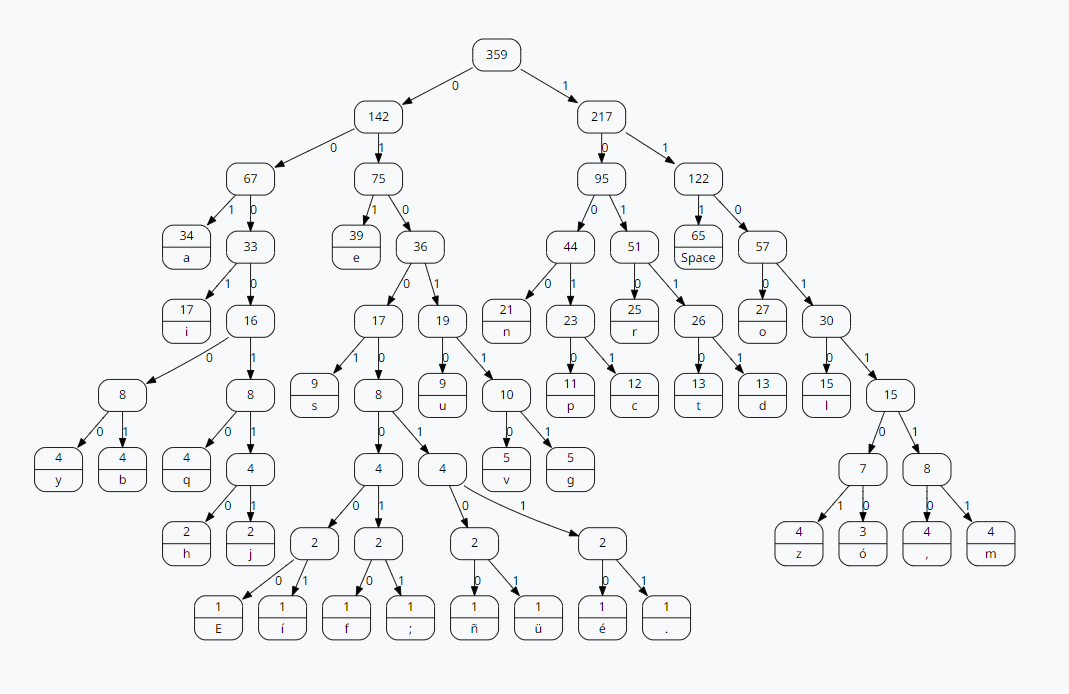
\includegraphics[width=14.9cm]{src/Img/ArbolHuffman.png}
    \end{center}

    Pero bueno por si acaso lo explico un poquito, hasta abajo vemos que los de frecuencia 1 se empezaron uniendo entre si generando arboles con raiz 2, a su vez se unieron entre si para generar arboles con raiz 4, aveces, cuando no hay arboles con la misma raiz, se toman los 2 de menor raiz digamos 8 y 9 se juntan para una raiz 17, y asi sucesivamente hasta que solo queda un arbol de raiz 359. \vspace{.2cm}

    Ahora, como mencionamos ir a la izquierda desde la raiz agrega un 0 a la codificacion del caracter y a la derecha un 1, entonces, si queremos saber la codificacion de una letra, simplemente seguimos el camino desde la raiz hasta la letra y anotamos los 0s y 1s que tomamos, este camino es unico aunque la codificacion no lo sea  (existen varias codificaciones de Huffman para este texto). Entonces por ejemplo el espacio tiene 111 como codificacion mientras que el . tiene una codificacion de 01000111 \vspace{.2cm} 
\end{quote}
    \item \textbf{Suponga que tenemos dos arreglos ordenados $A[1,\dots n]
\ y \ B[1, \dots, n]$ y un entero k. Describe un algoritmo para 
encontrar el \textit{k-ésimo} elemeneto en la unión de  \textit{A}
y \textit{B}. Por ejemplo, si $k=1$, tu algoritmo debe regresar el
elemento más pequeño de $A \cup B$; si $k=n$, tu algoritmo debe 
regresar la mediana de $A \cup B$. Puedes suponer que los arreglos 
no contienen duplicados. Tu algoritmo debe tener complejidad de tiempo
$\Theta (log \, n)$. Hint: Primero resuelve el caso especial k=n.}
    \item \textbf{Sea \textit{A} un arreglo de n númreos enteros distintos. Suponga
que \textit{A} tiene la siguiente propiedad: existe un indice $1 \leq k \leq
n$ tal que $A[1],\dots,A[k]$ es una secuencia incremental y $A[k+1],\dots,
A[n]$ es una secuencia decremental.}\\
    \begin{enumerate}
        \item \textbf{Describe un algoritmo que use $\Theta(n^2)$ comparaciones para resolver el problema.}\\

La primer idea es tomar cada contenedor de madera, llenarlo de sake y probar pasarlo hacia cada uno de los de vidrio contenedor $1$ hasta el $n$ de vidrio en el peor de los casos (obviamente tenemos que rellenarlo cada que no sean del mismo tamaño y no lo menciona pero supongo que también vaciar los contenedores de vidrio), esto en el peor de los casos nos toma n unidades de tiempo, ahora nos quedan n-1 contenedores de ambos tipos y repetimos, esto también esta en el orden de n unidades de tiempo y vamos a repetir para cada contenedor de madera, entonces la complejidad es $n+(n-1)+(n-2)\dots+1 = \frac{n(n+1)}{2} \in O(n^2)$ además podemos demostrar que tiene una cota superior si multiplicamos por ejemplo por 2 entonces $c_2=2$ y $\frac{n^2+x}{2} \leq 2*n^2$ y esto demuestra la cota superior $\forall n>1$, ahora tambien si tomamos $c_1=.1$ tenemos que $.1 n^2 \leq \frac{n^2+x}{2}$ $\forall n>1$ entonces demostrando que este algoritmo $\in \Theta(n^2)$.\\
        \item \textbf{Suponga por obvias razones, que solo nos interesa encontrar los contenedores que les cabe mas sake. Pruebe que esto puede hacerse con a lo mas 2n-2 comparaciones.}\\

Ahora, tomamos nuestro contenedor de madera, y comenzamos a rellenar y vertir en cada uno de los de vidrio, la idea es, buscar uno que le quepa mas que el que elegimos, en el peor de los casos comparamos nuestro botecito de madera con todos los y no fue hasta el ultimo que encontramos uno de vidrio que es mas grande (y no fue igual), afortunadamente ya solo quedan n-1 contenedores de madera así que comenzamos a comparar desde el segundo, en el peor de los casos, comparamos hasta llegar al penúltimo y este también es mas chico que nuestro bote de vidrio, es decir que ya sin comparar podemos saber que el ultimo contenedor de madera sera el que es de igual tamaño al que tenemos de vidrio y este par es el mas grande.\\

Para resumir el algoritmo, tomamos un contenedor de madera, el que sea, comparamos con cada uno de los de vidrio hasta llegar a uno mas grande (esto descarta los que comparaste antes) o acabemos con todos y solo a uno le cupo lo mismo (en cuyo caso acabaste), a la hora de intercambiar eliminamos los de madera que ya hayamos usado o comparado, de manera que seguimos con los que aun pueden ser mas grandes si encontramos uno mas grande otra vez alternamos y ahora usamos ese grande de madera para comparar con los de vidrio; notemos que recorremos el arreglo de los de vidrio hasta que no, tomamos el bote en el índice i+1 y recorremos los de madera 
desde el ultimo que usamos.\\

Como ya mencionamos esto en el peor de los casos recorre todos los de vidrio y después se pone a recorrer desde el segundo de madera hasta el penúltimo de madera (el primero lo usamos para comparar con los n de vidrio y el penúltimo no tiene caso comparar) así usando 2n-2 comparaciones para encontrar la pareja.\\
        \item \textbf{¿Puedes mejorar el numero de comparaciones esperadas del inciso a? Explica.}\\

Técnicamente podríamos usar algo como counting sort, fijándonos en vez del contenido que hay en los contenedores mas bien el contenido que queda en el barril de sake al llenar nuestro barril pero vamos a obviar esa respuesta.\\

Supongo que como se trata de un problema de ordenación, la cota mínima es $O(n log(n))$ pero en este caso sin información previa, no veo forma de hacer algo como merge sort o un árbol, en cualquier paso no podemos descartar parejas pues no podemos saber el orden de nuestros contenedores de madera con respecto a ellos mismos o los vidrio, por tanto para ordenarlos respecto a ellos mismos y al mismo tiempo respecto al otro grupo se necesitaran $O(n^2)$ comparaciones.
    \end{enumerate}
    \item \textbf{Usted tiene que ordenar una serie $\Sigma_n$ de $n$ números, tales que todos son 0 ó 1. La única operación que puede hacer es comparar dos números cualesquiera $x$ y $y$, y cada que los compara recibe la respuesta $x < y$, $x = y$, or $x > y$.}\vspace{.2cm}
    \item \textbf{Se dice que un arreglo A[1,...,n] es k-ordenado si este puede ser dividido en k bloques cada uno de tamaño $\frac{n}{k}$ aproximadamente, tal que todos los elementos en cada bloque son mas grandes que el bloque anterior y mas pequeños que los elementos del bloque siguiente. Los elementos en cada bloque podrían no estar ordenados. Por ejemplo, el siguiente arreglo es 4-ordenado:
\begin{align*}
    1,2,4,3 \,|\, 7,6,5 \,|\, 10,11,9,12 \,|\, 15,13,16,14\\
\end{align*}}


    \begin{enumerate}
        \item \textbf{Describe un algoritmo que k-ordene un arreglo de tamaño n en tiempo $O(n \, logk)$.}\\

Para este problema vamos a utilizar una versión modificada de \textbf{Quick sort} pero además vamos a utilizar la versión que toma su pivote con la mediana en tiempo O(n) para asegurar la complejidad en el peor de los casos.\\

\textcolor{bibi}{Quick sort}
\begin{quote}
    Lo primero que nos interesa es que dividamos el arreglo en $k$ bloques, pero como estamos usando quick sort modificado, lo primero es encontrar la mediana en $O(n)$, una vez encontrada esta mediana tenemos un buen pivote, podemos comenzar a dividir, en este paso vamos a tener 2 fracciones de n, probablemente no estén cerca de ser $n/2$ pero si sabemos que serán algo como $n/c_1$ y $n/c_2$.\\

    En el siguiente paso, de nuevo buscamos la mediana en cada fracción en tiempo $O(n)$ y obtenemos de nuevo una fracción de n (asegurado por buscar la mediana); esto lo vamos a repetir hasta que el árbol llegue a arreglos de tamaño $n/k$ como lo estamos dividiendo en fracciones de $n$ entonces la altura del árbol binario implícito va a ser logarítmica, ahora vamos a checar cual es la altura de dicho árbol, en cada paso van a ser fracciones diferentes pero como queremos hacernos el calculo mas fácil en promedio podemos decir que se van a dividir en una fracción $1/c$ con c constante (en verdad c cambia en cada paso pero su valor es poco relevante). Entonces la altura del árbol la vamos a calcular de la siguiente manera, comenzamos con n elementos y luego vamos partiendo por nuestro c hasta que lleguemos a k grupos de tamaño $n/k$:
    \begin{align*}
        n, \frac{n}{c}, \frac{n}{c^2}, \dots, \frac{n}{c^m} = \frac{n}{k} \xrightarrow{} kn &= c^m * n \\
        k &= c^m \\
        log_c{\ k} &= log_c{\ c^m} \\
        log_c{\ k} &= m
    \end{align*}

    Notemos que los valores de C en realidad no alteran mas que la base del logaritmo y además m representaba el nivel de profundidad del árbol, es decir tras m niveles del árbol que dividía en fracciones de n tendremos k grupos de tamaño aproximado $n/k$.\\

    Entonces, sabemos que para cada nivel del árbol, buscaremos la mediana de las medianas que se puede hacer en $O(n)$ además de que vamos a recorrer todo el arreglo que también esta en $O(n)$; simplificando cada nivel hace una cantidad lineal de operaciones; después vimos que vamos a estar dividiendo (gracias a la mediana de las medianas) a n en una fracción de si misma por cada nivel y además dividiremos hasta que lleguemos a arreglos de tamaño $n/k$ de manera que tendremos $log_C(\ k)$ niveles, multiplicando estas complejidades tenemos que $O(n(log_C(\ k))) = O(n \ log(k))$, aunque hay que aclarar que las constantes ocultas probablemente son muy grandes especialmente estar calculando mediana de medianas en todos los pasos.\\
\end{quote}
        \item \textbf{What is a good strategy is $n$ is not known?}\vspace{.2cm}

\textcolor{bibi}{}
\begin{quote}
\end{quote}
    \end{enumerate}
    \item \textbf{Considera el siguiente algoritmo para ordenar:
\begin{center}
        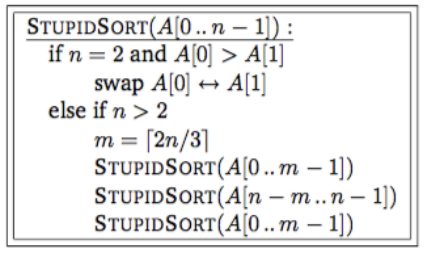
\includegraphics[width=5cm]{src/Img/stupidSort.png}\\
\end{center}}

    \begin{enumerate}
        \item \textbf{
    Supongamos que la capacidad de una sola arista $e$ se incrementa en una unidad. De un 
    algoritmo de tiempo $O(n+E)$ para actualizar nuestro flujo. $E$ es el número de aristas 
    de $N$.
}\vspace{.2cm}
\textcolor{bibi}{}
\begin{quote}
\end{quote}
        \item \textbf{
    Supongamos que la capacidad de una sola arista $e$ se decrementa en una unidad. De un
    algoritmo de tiempo $O(n + E)$ donde $E$ es el número de aristas de $N$.
}\vspace{.2cm}
\textcolor{bibi}{}
\begin{quote}
\end{quote}
        \item \textbf{Demuestra que el numero de "swaps" hechos por STUPIDSORT es a lo mas $\binom{n}{2}$.}\\

Lo importante para demostrar esto y por falta de tiempo es que el algoritmo solo mete parejas de números una vez y es que notemos que si mete una pareja digamos (i,j) eso significa que $i<j$ o al revés, en cualquier caso los swapea una sola vez y después de esto no puede darse el caso de que vuelva a meter a la pareja (i,j) pues significaría que $j<i$ que no hay forma que suceda; entonces si consideramos $\binom{n}{2}$ es decir tomar de n números parejas de 2 en 2, ya estamos considerando todos los casos posibles de parejas lo cual sucede en el peor de los casos.\\


    \end{enumerate}
    \item \textbf{Dado un arreglo $A$ con $n$ enteros positivos y negativos.}\vspace{.2cm}

\textcolor{bibi}{}
\begin{quote}
\end{quote}
    \begin{enumerate}
        \item \textbf{Suponiendo que puede cambiar de posición a las personas ¿Se puede resolver el problema con a lo mas una orden? Explique.}\\

Si, asumiendo que el mover de posición no cuenta como una orden, seria poner a todos los que tengan de una forma de un lado y los que lo tengan de la otra del lado contrario, así podríamos dar la orden de tomar uno de los 2 lados y pedirles a todos hasta el ultimo de esa forma que se cambien la gorra hacia el lado opuesto y tendríamos a todos de manera uniforme, (no se si entendí bien esta pregunta xd).\\
        \item \textbf{Dise\~na un algoritmo de programaci\'on din\'amica eficiente que determine si $Z$ es un \textit{shuffle} de $X$ y $Y$. \textit{Hint}: Los valores de la matriz de programaci\'on din\'amica que construyas, podr\'ian ser valores booleanos y no num\'ericos.}\vspace{.2cm}

El problema se parece bastante a la subcadena creciente mas grande.
La idea es usar una matriz de $|X|+1$ filas y $|Y|+1$ columnas, 
donde la celda $(i,j)$ indica si los primeros $i+j$ caracteres de $Z$
son un \textit{shuffle} de los primeros $j$ caracteres de $X$ y 
los primeros $i$ caracteres de $Y$. (podemos cambiar cual es quien pero asi lo hice) \vspace{.2cm}
    
\textcolor{bibi}{Usando matriz y programaci\'on din\'amica:}\vspace{.2cm}
\begin{quote}

    Podemos empezar verificando que $|X|+|Y|=|Z|$, si no es asi entonces
    no puede ser un \textit{shuffle} de $X$ y $Y$. \vspace{.2cm}

    Tenemos entonces que nuestra matriz se va a ver algo as\'i:

    \begin{table}[H]
        \centering
        \begin{tabular}{lllllll}
                &                              &                       & $x_0$                 & $x_1$                 & $\dots$               & $x_n$                 \\
                & i/j                          & 0                     & 1                     & 1                     & $\dots$               & n                     \\ \cline{3-7} 
                & \multicolumn{1}{l|}{0}       & \multicolumn{1}{l|}{1} & \multicolumn{1}{l|}{} & \multicolumn{1}{l|}{} & \multicolumn{1}{l|}{} & \multicolumn{1}{l|}{} \\ \cline{3-7} 
        $y_0$   & \multicolumn{1}{l|}{1}       & \multicolumn{1}{l|}{} & \multicolumn{1}{l|}{} & \multicolumn{1}{l|}{} & \multicolumn{1}{l|}{} & \multicolumn{1}{l|}{} \\ \cline{3-7} 
        $y_1$   & \multicolumn{1}{l|}{2}       & \multicolumn{1}{l|}{} & \multicolumn{1}{l|}{} & \multicolumn{1}{l|}{} & \multicolumn{1}{l|}{} & \multicolumn{1}{l|}{} \\ \cline{3-7} 
        $\dots$ & \multicolumn{1}{l|}{$\dots$} & \multicolumn{1}{l|}{} & \multicolumn{1}{l|}{} & \multicolumn{1}{l|}{} & \multicolumn{1}{l|}{} & \multicolumn{1}{l|}{} \\ \cline{3-7} 
        $y_m$   & \multicolumn{1}{l|}{m}       & \multicolumn{1}{l|}{} & \multicolumn{1}{l|}{} & \multicolumn{1}{l|}{} & \multicolumn{1}{l|}{} & \multicolumn{1}{l|}{} \\ \cline{3-7} 
        \end{tabular}
    \end{table}

    Ahora vamos a ver como llenarla, primero por la definición que hicimos, el indice
    (i,j) sera 1 pues los primeros 0+0 caracteres de Z siempre seran shuffle de los primeros
    0 caracteres de X y los primeros 0 caracteres de Y. \vspace{.2cm}

    Para la primera fila, hay que checar que los primeros $j$ caracteres de $X$ sean iguales
    a los primeros $j$ caracteres de $Z$, si es asi, entonces la celda $(0,j)$ sera 1, si no
    entonces sera 0; para checar esto podemos checar si el caracter j es igual en ambos y despues
    checar si a la izquierda ya tenemos un 1. ( esto es equivalente a: M[0][j]=M[0][j-1] AND X[j-1]==Z[j-1]
    tenemos que restar 1 porque las cadenas tienen indice en 0 pero tambien lo puedes entender con cantidad
    de caracteres) \vspace{.2cm}

    Para la primera columna, es lo mismo que la fila pero con $Y$ y $Z$, esto se puede entender como
    M[i][0]=M[i-1][0] AND Y[i-1]==Z[i-1]. \vspace{.2cm}

    Ahora para el caso de en medio hay que checar que los primeros $i+j$ caracteres de $Z$ sean shuffle
    de los primeros $j$ caracteres de $X$ y los primeros $i$ caracteres de $Y$, esto se puede entender
    como M[i][j]=M[i-1][j] AND Y[i-1]==Z[i+j-1] OR M[i][j-1] AND X[j-1]==Z[i+j-1]. \vspace{.2cm}

    De manera general nuestra funcion quedaria algo asi:
    \scriptsize
    \begin{align*}
        M[i][j]=\begin{cases}
            1 & \text{si } i=0 \text{ y } j=0 \\
            (M[i-1][j] \text{ AND } Y[i-1]==Z[i+j-1]) \text{ OR } (M[i][j-1] \text{ AND } X[j-1]==Z[i+j-1]) & \text{si } i>0 \text{ y } j>0 \\
        \end{cases}
    \end{align*}

    Al final sabremos si $Z$ es un \textit{shuffle} de $X$ y $Y$ si $M[|Y|][|X|]=1$, ademas el camino
    para ir de la celda $(|Y|,|X|)$ a la celda $(0,0)$ nos dira cuales son los caracteres que se usaron. \vspace{.2cm}

    Este algoritmo tiene complejidad $O(|X|*|Y|)$ y usa $O(|X|*|Y|)$ memoria, esto pues la matriz es de tamaño
    $(|X|+1)*(|Y|+1)$ y se llena en cada celda una vez tomando $O(1)$ tiempo (checar arriba y abajo, tomar un indice de 
    una cadena y compararlo con el indice en otra cadena que puede ser O(1)). \vspace{.2cm}

    Para entender mejor checar el ejemplo de arriba.
\end{quote}


\newpage
        \item \textbf{Suponiendo que no puede cambiar de posición a las personas. Diseñe un algoritmo de tiempo lineal tal que todos los asistentes tengan la visera del mismo lado al ingresar pero garantice el mínimo numero de cambios.}\\

En este caso primero vamos a contar la cantidad que lo tiene de cada forma, (de nuevo no se si contamos esto como algo pero sube la complejidad implementándolo) esto ocupa 0 ordenes o cambios, una vez contado esto solo hay que recorrer la lista y pedirles a los que tuvieron la forma menos común, que se giren la gorra.
    \end{enumerate}
\end{enumerate}

\end{document}